\documentclass[12pt,a4paper]{article}
\usepackage[utf8]{vietnam}
\usepackage{amsmath,amssymb}
\usepackage{tabularx}
\usepackage{tikz}
\usetikzlibrary{calc,angles,quotes,arrows.meta,patterns}
\usepackage{xcolor}
\usepackage{enumitem}
\usepackage{fancyhdr}
\usepackage[top=1.0cm, bottom=1.1cm, left=1.3cm, right=1.3cm]{geometry}
\usepackage[dethi]{ex_test}

\setlength{\headheight}{15pt}
\setlength{\parskip}{1.5pt}

\pagestyle{fancy}
\fancyhf{}
\lhead{\textit{Chuyên đề: Tam giác bằng nhau \& Toán đố Phân số -- Toán 7}}
\rhead{\textit{Tài liệu bồi dưỡng đa dạng phương pháp giải}}
\cfoot{\thepage/4}

\begin{document}

% =============================================================================
% TRANG 1: TIÊU ĐỀ & ĐỀ BÀI & BÀI 1
% =============================================================================
\begin{center}
  {\bfseries\large HƯỚNG DẪN GIẢI CHI TIẾT VÀ PHÂN TÍCH ĐA DẠNG PHƯƠNG PHÁP}\\
  \vspace{1mm}
  {\bfseries\Large BÀI TẬP HÌNH HỌC VÀ SỐ HỌC TOÁN 7}\\
  \vspace{1mm}
  \textit{(Tài liệu bồi dưỡng học sinh -- Phân tích sâu theo chuẩn phương pháp sư phạm)}
\end{center}
\vspace{-2mm}
\hrule
\vspace{2mm}

\noindent\textbf{\large A. TỔNG HỢP ĐỀ BÀI (TỪ ẢNH CHỤP VỞ HỌC SINH)}

\begin{enumerate}[label=\textbf{Bài \arabic*.}, leftmargin=*, itemsep=2pt, parsep=0pt]
  \item Cho $\Delta ABC = \Delta MNP$ có $AB = 5\,\text{cm}$, $AC = 7\,\text{cm}$, $NP = (2x + 1)\,\text{cm}$ và chu vi tam giác $ABC$ bằng $21\,\text{cm}$. Tìm $x$.
  \item Một thùng chứa $120$ lít nước, lần thứ nhất người ta dùng $\dfrac{1}{4}$ lượng nước trong thùng; lần thứ hai dùng $\dfrac{2}{5}$ lượng nước còn lại sau lần thứ nhất. Hỏi sau hai lần dùng, trong thùng còn bao nhiêu lít nước?
  \item Cho tam giác $ABC$. Trên nửa mặt phẳng bờ $AC$ không chứa điểm $B$, lấy điểm $D$ sao cho $AD = BC$ và $CD = AB$.
  Vẽ hình và ghi giả thiết, kết luận của bài toán; sau đó:
  \textbf{a)} Chứng minh $\Delta ABC = \Delta CDA$;
  \textbf{b)} Chứng minh $AB \parallel CD$;
  \textbf{c)} Cho $\widehat{BAC} = 50^\circ$ và $\widehat{ABC} = 60^\circ$. Tính số đo $\widehat{ACB}$.
\end{enumerate}

\vspace{1.5mm}
\hrule
\vspace{2mm}

\noindent\textbf{\large B. LỜI GIẢI CHI TIẾT VÀ ĐA DẠNG PHƯƠNG PHÁP TIẾP CẬN}

\vspace{1.5mm}
\noindent\textbf{\large 1. BÀI TOÁN 1: TÌM ẨN SỐ TRONG TAM GIÁC BẰNG NHAU}

\noindent\textbf{\textit{Phân tích cốt lõi:}} Ký hiệu $\Delta ABC = \Delta MNP$ quy định thứ tự các đỉnh tương ứng: $A \leftrightarrow M$, $B \leftrightarrow N$, $C \leftrightarrow P$.
Suy ra các cạnh tương ứng bằng nhau:
\[
  AB = MN = 5\,\text{cm}, \quad AC = MP = 7\,\text{cm}, \quad BC = NP = (2x + 1)\,\text{cm}.
\]

\noindent\textbf{$\blacktriangleright$ Cách 1 (Phương pháp đại số cơ bản -- Chuẩn mực SGK):}
\begin{itemize}[leftmargin=16pt, itemsep=1.5pt, parsep=0pt]
  \item Chu vi tam giác $ABC$ là: $C_{\Delta ABC} = AB + AC + BC = 21\,\text{cm}$.
  \item Độ dài cạnh $BC$ là: $BC = 21 - AB - AC = 21 - 5 - 7 = 9\,\text{(cm)}$.
  \item Vì $\Delta ABC = \Delta MNP$ nên hai cạnh tương ứng $NP = BC$. Ta có phương trình:
  \[
    2x + 1 = 9 \iff 2x = 9 - 1 \iff 2x = 8 \iff x = 4.
  \]
  \item \textbf{Kết luận:} Vậy $x = 4$.
\end{itemize}

\noindent\textbf{$\blacktriangleright$ Cách 2 (Dùng tính chất chu vi hai tam giác bằng nhau):}
\begin{itemize}[leftmargin=16pt, itemsep=1.5pt, parsep=0pt]
  \item Vì $\Delta ABC = \Delta MNP$ nên chu vi của chúng bằng nhau: $C_{\Delta MNP} = C_{\Delta ABC} = 21\,\text{cm}$.
  \item Các cạnh của $\Delta MNP$: $MN = AB = 5\,\text{cm}$, $MP = AC = 7\,\text{cm}$, $NP = (2x + 1)\,\text{cm}$.
  \item Chu vi $\Delta MNP$ là tổng 3 cạnh:
  \[
    5 + 7 + (2x + 1) = 21 \iff 2x + 13 = 21 \iff 2x = 8 \iff x = 4.
  \]
\end{itemize}

\noindent\textbf{$\blacktriangleright$ Cách 3 (Sơ đồ số học trực quan):}
\begin{itemize}[leftmargin=16pt, itemsep=1.5pt, parsep=0pt]
  \item Tổng hai cạnh đã biết: $5 + 7 = 12\,\text{cm}$.
  \item Cạnh còn lại $NP$ là: $21 - 12 = 9\,\text{cm}$.
  \item Ta tìm $x$ sao cho: $2 \times x + 1 = 9 \implies 2 \times x = 8 \implies x = 4$.
\end{itemize}

\noindent\textbf{$\blacktriangleright$ Kiểm tra điều kiện hình học (Bất đẳng thức tam giác):}
Với $x = 4$, ba cạnh là $5\,\text{cm}, 7\,\text{cm}, 9\,\text{cm}$. Ta có $5 + 7 = 12 > 9$; $5 + 9 = 14 > 7$; $7 + 9 = 16 > 5$ (luôn thỏa mãn).

\noindent\textbf{\textit{\textbf{[Lưu ý]} Sai lầm học sinh thường gặp:}}
\begin{itemize}[leftmargin=16pt, itemsep=1pt, parsep=0pt]
  \item Nhầm cạnh tương ứng: gán nhầm $NP = AB = 5$ hoặc $NP = AC = 7$, dẫn tới $x = 2$ hoặc $x = 3$.
  \item Nhầm cạnh $NP$ với chu vi: giải $2x + 1 = 21 \implies x = 10$.
\end{itemize}

\newpage

% =============================================================================
% TRANG 2: BÀI 2
% =============================================================================
\noindent\textbf{\large 2. BÀI TOÁN 2: TOÁN THỰC TẾ VỀ PHÂN SỐ CỦA MỘT SỐ}

\vspace{1mm}
\noindent\textbf{\textit{Phân tích từ khóa mấu chốt:}} Lần 2 dùng $\dfrac{2}{5}$ lượng nước \textbf{CÒN LẠI sau lần thứ nhất} (chứ không phải của lượng nước ban đầu $120$ lít).

\vspace{2mm}
\noindent\textbf{$\blacktriangleright$ Cách 1 (Số học cụ thể từng bước -- Tự nhiên, dễ hiểu nhất):}
\begin{enumerate}[label=\arabic*), leftmargin=18pt, itemsep=2pt, parsep=0pt]
  \item Lượng nước dùng lần thứ nhất là:
  \[
    120 \times \frac{1}{4} = 30\,\text{(lít)}.
  \]
  \item Lượng nước còn lại trong thùng sau lần dùng thứ nhất là:
  \[
    120 - 30 = 90\,\text{(lít)}.
  \]
  \item Lượng nước dùng lần thứ hai là:
  \[
    90 \times \frac{2}{5} = 36\,\text{(lít)}.
  \]
  \item Lượng nước còn lại trong thùng sau hai lần dùng là:
  \[
    90 - 36 = 54\,\text{(lít)} \quad (\text{hoặc } 120 - 30 - 36 = 54\,\text{lít}).
  \]
\end{enumerate}
\textbf{Đáp số:} $54$ lít.

\vspace{2.5mm}
\noindent\textbf{$\blacktriangleright$ Cách 2 (Tìm phân số chỉ lượng còn lại -- Nhân phân số liên tiếp, tinh gọn nhất):}
\begin{itemize}[leftmargin=16pt, itemsep=2pt, parsep=0pt]
  \item Sau lần 1, lượng nước còn lại chiếm: $1 - \dfrac{1}{4} = \dfrac{3}{4}$ (lượng nước ban đầu).
  \item Lần 2 dùng $\dfrac{2}{5}$ lượng còn lại, nên sau lần 2 lượng nước còn lại chiếm:
  $1 - \dfrac{2}{5} = \dfrac{3}{5}$ (lượng nước sau lần 1).
  \item Phân số chỉ lượng nước còn lại sau hai lần so với lượng nước ban đầu là:
  \[
    \frac{3}{4} \times \frac{3}{5} = \frac{9}{20} \text{ (lượng nước ban đầu)}.
  \]
  \item Số lít nước còn lại trong thùng là:
  \[
    120 \times \frac{9}{20} = 54\,\text{(lít)}.
  \]
\end{itemize}

\vspace{2.5mm}
\noindent\textbf{$\blacktriangleright$ Cách 3 (Phương pháp sơ đồ đoạn thẳng trực quan):}
\begin{center}
\begin{tikzpicture}[scale=0.95, >=stealth]
  % Thanh 1: Ban dau 120 lit
  \draw[thick] (0,0) rectangle (12,0.65);
  \node at (6, 0.32) {\footnotesize 120 lít nước ban đầu (chia làm 20 phần bằng nhau, mỗi phần = 6 lít)};
  
  % Thanh 2: Sau Lan 1
  \fill[blue!15] (0,-1.15) rectangle (3,-0.55);
  \fill[gray!10] (3,-1.15) rectangle (12,-0.55);
  \draw[thick] (0,-1.15) rectangle (12,-0.55);
  \draw[thick, dashed] (3,-1.15) -- (3,-0.55);
  \node at (1.5, -0.85) {\scriptsize Lần 1: 30 lít (5 phần)};
  \node at (7.5, -0.85) {\scriptsize Còn lại sau Lần 1: 90 lít (15 phần)};
  
  % Thanh 3: Sau Lan 2
  \fill[gray!20] (0,-2.0) rectangle (3,-1.4);
  \fill[orange!20] (3,-2.0) rectangle (6.6,-1.4);
  \fill[green!25] (6.6,-2.0) rectangle (12,-1.4);
  \draw[thick] (0,-2.0) rectangle (12,-1.4);
  \draw[thick, dashed] (3,-2.0) -- (3,-1.4);
  \draw[thick, dashed] (6.6,-2.0) -- (6.6,-1.4);
  \node at (1.5, -1.7) {\scriptsize Đã dùng L1 (30l)};
  \node at (4.8, -1.7) {\scriptsize Lần 2: 36 lít (6 phần)};
  \node at (9.3, -1.7) {\bfseries\footnotesize Còn lại: 54 lít (9 phần)};
\end{tikzpicture}
\end{center}

\vspace{1.5mm}
\noindent\textbf{$\blacktriangleright$ Cách 4 (Quy đổi tỉ số phần trăm):}
\begin{itemize}[leftmargin=16pt, itemsep=1.5pt, parsep=0pt]
  \item Lần 1 dùng $\dfrac{1}{4} = 25\%$, còn lại: $100\% - 25\% = 75\%$ lượng ban đầu.
  \item Lần 2 dùng $\dfrac{2}{5} = 40\%$ của $75\%$, chiếm: $40\% \times 75\% = 30\%$ lượng ban đầu.
  \item Lượng nước còn lại chiếm: $75\% - 30\% = 45\%$ lượng ban đầu.
  \item Số lít nước còn lại là: $120 \times 45\% = 120 \times 0{,}45 = 54$ (lít).
\end{itemize}

\vspace{1.5mm}
\noindent\textbf{\textit{\textbf{[Lưu ý]} Bẫy sai lầm kinh điển cần tránh:}}
Học sinh lấy $\dfrac{2}{5} \times 120 = 48$ lít rồi lấy $120 - 30 - 48 = 42$ lít (\textbf{SAI HOÀN TOÀN} do không nhân với lượng còn lại).

\newpage

% =============================================================================
% TRANG 3: BÀI 3 (HÌNH VẼ, GT-KL, CÂU A, CÂU B)
% =============================================================================
\noindent\textbf{\large 3. BÀI TOÁN 3: HÌNH HỌC TAM GIÁC BẰNG NHAU VÀ ĐƯỜNG SONG SONG}

\vspace{2mm}
\noindent
\begin{minipage}[t]{0.56\linewidth}
\textbf{Giả thiết và Kết luận chuẩn mực:}\\[1.5mm]
\begin{tabular}{|l|p{6.1cm}|}
\hline
\textbf{GT} & $\Delta ABC$; Điểm $D$ thuộc nửa mặt phẳng bờ $AC$ không chứa $B$; \\
& $AD = BC$; $CD = AB$; \\
& $\widehat{BAC} = 50^\circ$; $\widehat{ABC} = 60^\circ$ (cho câu c). \\
\hline
\textbf{KL} & a) $\Delta ABC = \Delta CDA$. \\
& b) $AB \parallel CD$. \\
& c) Tính số đo $\widehat{ACB}$. \\
\hline
\end{tabular}
\end{minipage}\hfill
\begin{minipage}[t]{0.42\linewidth}
\vspace{-3mm}
\begin{center}
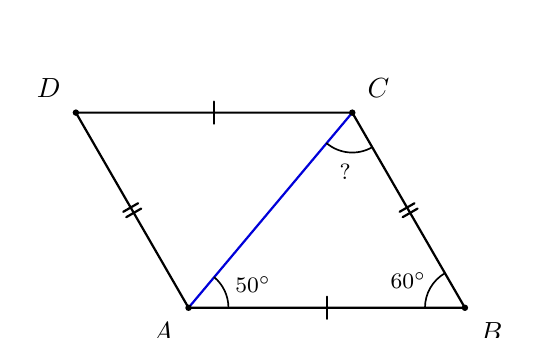
\begin{tikzpicture}[scale=0.78, >=stealth, line cap=round, line join=round]
  \coordinate (A) at (0,0);
  \coordinate (B) at (4.5,0);
  \coordinate (C) at (2.666, 3.177);
  \coordinate (D) at (-1.834, 3.177);
  
  % Canh tu giac va duong cheo AC
  \draw[thick] (A) -- (B) -- (C) -- (D) -- cycle;
  \draw[thick, blue!85!black] (A) -- (C);
  
  % Dinh va nhan dinh
  \fill (A) circle (1.5pt) node[below left=2pt] {$A$};
  \fill (B) circle (1.5pt) node[below right=2pt] {$B$};
  \fill (C) circle (1.5pt) node[above right=2pt] {$C$};
  \fill (D) circle (1.5pt) node[above left=2pt] {$D$};
  
  % Ki hieu doan bang nhau AB = CD (1 gach vuong goc)
  \draw[thick] (2.25, -0.18) -- (2.25, 0.18);
  \draw[thick] (0.416, 2.997) -- (0.416, 3.357);
  
  % Ki hieu doan bang nhau AD = BC (2 gach vuong goc)
  % Doan AD
  \draw[thick] (-0.892 - 0.14*0.866, 1.545 - 0.14*0.5) -- (-0.892 + 0.14*0.866, 1.545 + 0.14*0.5);
  \draw[thick] (-0.942 - 0.14*0.866, 1.632 - 0.14*0.5) -- (-0.942 + 0.14*0.866, 1.632 + 0.14*0.5);
  % Doan BC
  \draw[thick] (3.608 - 0.14*0.866, 1.545 - 0.14*0.5) -- (3.608 + 0.14*0.866, 1.545 + 0.14*0.5);
  \draw[thick] (3.558 - 0.14*0.866, 1.632 - 0.14*0.5) -- (3.558 + 0.14*0.866, 1.632 + 0.14*0.5);
  
  % Cung goc BAC = 50 do
  \draw[semithick] (A) ++(0:0.65) arc (0:50:0.65);
  \node at (1.05, 0.38) {\footnotesize $50^\circ$};
  
  % Cung goc ABC = 60 do
  \draw[semithick] (B) ++(180:0.65) arc (180:120:0.65);
  \node at (3.58, 0.44) {\footnotesize $60^\circ$};
  
  % Cung goc ACB can tinh (?)
  \draw[semithick] (C) ++(230:0.65) arc (230:300:0.65);
  \node at (2.55, 2.22) {\footnotesize $?$};
\end{tikzpicture}
\end{center}
\end{minipage}

\vspace{2mm}
\noindent\textbf{a) Chứng minh $\Delta ABC = \Delta CDA$:}
\begin{itemize}[leftmargin=16pt, itemsep=2pt, parsep=0pt]
  \item Xét tam giác $ABC$ và tam giác $CDA$, ta có:
  \begin{itemize}[leftmargin=14pt, itemsep=1.5pt]
    \item $AB = CD$ (theo giả thiết).
    \item $BC = DA$ (theo giả thiết, vì $AD = BC$).
    \item $AC$ là cạnh chung.
  \end{itemize}
  \item Do đó:
  \[
    \Delta ABC = \Delta CDA \quad (\text{cạnh -- cạnh -- cạnh}).
  \]
  \item \textbf{\textit{Quy tắc thứ tự đỉnh tương ứng bắt buộc:}}
  $A$ đối diện cạnh $BC$, tương ứng với $C$ đối diện cạnh $AD$ ($A \leftrightarrow C$).
  $B$ đối diện $AC$, tương ứng với $D$ đối diện $CA$ ($B \leftrightarrow D$).
  Do đó bắt buộc viết: $\Delta ABC = \Delta CDA$ (viết $\Delta ABC = \Delta CAD$ là \textbf{sai}).
\end{itemize}

\vspace{3mm}
\noindent\textbf{b) Chứng minh $AB \parallel CD$:}

\noindent\textbf{$\blacktriangleright$ Cách 1 (Dùng cặp góc so le trong bằng nhau -- Cách tối ưu và trực tiếp nhất):}
\begin{itemize}[leftmargin=16pt, itemsep=1.5pt, parsep=0pt]
  \item Từ kết quả câu a: $\Delta ABC = \Delta CDA$, suy ra:
  \[
    \widehat{BAC} = \widehat{DCA} \text{ (hai góc tương ứng)}.
  \]
  \item Vì điểm $B$ và $D$ nằm trên hai nửa mặt phẳng đối nhau bờ $AC$, nên hai góc $\widehat{BAC}$ và $\widehat{DCA}$ ở vị trí \textbf{so le trong} tạo bởi cát tuyến $AC$ với hai đường thẳng $AB$ và $CD$.
  \item Theo dấu hiệu nhận biết hai đường thẳng song song, suy ra:
  \[
    AB \parallel CD \quad (\text{đpcm}).
  \]
\end{itemize}

\noindent\textbf{$\blacktriangleright$ Cách 2 (Kẻ đường chéo phụ $BD$):}
\begin{itemize}[leftmargin=16pt, itemsep=1.5pt, parsep=0pt]
  \item Nối đoạn thẳng $BD$. Xét $\Delta ABD$ và $\Delta CDB$ có:
  $AB = CD$ (gt), $AD = CB$ (gt), $BD$ là cạnh chung.
  \item Suy ra: $\Delta ABD = \Delta CDB$ (c.c.c) $\implies \widehat{ABD} = \widehat{CDB}$ (hai góc tương ứng).
  \item Hai góc này ở vị trí so le trong đối với cát tuyến $BD$, do đó $AB \parallel CD$.
\end{itemize}

\noindent\textbf{$\blacktriangleright$ Cách 3 (Phương pháp phản chứng logic):}
\begin{itemize}[leftmargin=16pt, itemsep=1.5pt, parsep=0pt]
  \item Giả sử $AB$ không song song với $CD$, khi đó chúng cắt nhau tại điểm $O$.
  \item Trong tam giác $OAC$, cát tuyến $AC$ tạo ra góc trong và góc ngoài không kề bằng nhau ($\widehat{BAC} = \widehat{DCA}$), điều này mâu thuẫn với định lí góc ngoài tam giác. Vậy $AB \parallel CD$.
\end{itemize}

\newpage

% =============================================================================
% TRANG 4: CÂU C & MỞ RỘNG
% =============================================================================
\noindent\textbf{c) Tính số đo $\widehat{ACB}$ khi $\widehat{BAC} = 50^\circ$ và $\widehat{ABC} = 60^\circ$:}

\vspace{1.5mm}
\noindent\textbf{$\blacktriangleright$ Cách 1 (Áp dụng định lí tổng ba góc trong $\Delta ABC$ -- Nhanh và chuẩn nhất):}
\begin{itemize}[leftmargin=16pt, itemsep=2pt, parsep=0pt]
  \item Xét $\Delta ABC$, theo định lí tổng ba góc trong một tam giác:
  \[
    \widehat{BAC} + \widehat{ABC} + \widehat{ACB} = 180^\circ.
  \]
  \item Thay số:
  \[
    50^\circ + 60^\circ + \widehat{ACB} = 180^\circ \implies 110^\circ + \widehat{ACB} = 180^\circ \implies \widehat{ACB} = 180^\circ - 110^\circ = 70^\circ.
  \]
  \item \textbf{Kết luận:} Vậy $\widehat{ACB} = 70^\circ$.
\end{itemize}

\vspace{1.5mm}
\noindent\textbf{$\blacktriangleright$ Cách 2 (Sử dụng tính chất góc ngoài của tam giác):}
\begin{itemize}[leftmargin=16pt, itemsep=2pt, parsep=0pt]
  \item Kẻ tia đối $Cx$ của tia $CB$. Góc $\widehat{ACx}$ là góc ngoài tại đỉnh $C$ của tam giác $ABC$:
  \[
    \widehat{ACx} = \widehat{BAC} + \widehat{ABC} = 50^\circ + 60^\circ = 110^\circ.
  \]
  \item Vì $\widehat{ACB}$ và $\widehat{ACx}$ là hai góc kề bù, nên:
  \[
    \widehat{ACB} = 180^\circ - \widehat{ACx} = 180^\circ - 110^\circ = 70^\circ.
  \]
\end{itemize}

\vspace{1.5mm}
\noindent\textbf{$\blacktriangleright$ Cách 3 (Tính gián tiếp thông qua tam giác bằng nhau $\Delta CDA$):}
\begin{itemize}[leftmargin=16pt, itemsep=2pt, parsep=0pt]
  \item Vì $\Delta ABC = \Delta CDA$ (chứng minh ở câu a), nên:
  \[
    \widehat{CDA} = \widehat{ABC} = 60^\circ \quad \text{và} \quad \widehat{DCA} = \widehat{BAC} = 50^\circ.
  \]
  \item Trong tam giác $CDA$: $\widehat{CAD} = 180^\circ - (\widehat{CDA} + \widehat{DCA}) = 180^\circ - (60^\circ + 50^\circ) = 70^\circ$.
  \item Do hai tam giác bằng nhau nên hai góc tương ứng bằng nhau: $\widehat{ACB} = \widehat{CAD} = 70^\circ$.
\end{itemize}

\vspace{1.5mm}
\noindent\textbf{$\blacktriangleright$ Cách 4 (Dùng tính chất hai đường thẳng song song và hai góc trong cùng phía):}
\begin{itemize}[leftmargin=16pt, itemsep=2pt, parsep=0pt]
  \item Chứng minh tương tự câu b, ta cũng có $\widehat{BCA} = \widehat{DAC}$ (so le trong) $\implies AD \parallel BC$.
  \item Vì $AD \parallel BC$, hai góc trong cùng phía bù nhau:
  $\widehat{DAB} + \widehat{ABC} = 180^\circ \implies \widehat{DAB} = 180^\circ - 60^\circ = 120^\circ$.
  \item Mà $\widehat{DAB} = \widehat{BAC} + \widehat{CAD} \implies \widehat{CAD} = 120^\circ - 50^\circ = 70^\circ \implies \widehat{ACB} = \widehat{CAD} = 70^\circ$.
\end{itemize}

\vspace{2mm}
\hrule
\vspace{2mm}

\noindent\textbf{\large C. BÀI TOÁN PHÁT TRIỂN VÀ MỞ RỘNG TƯ DUY NÂNG CAO}

\begin{enumerate}[label=\textbf{\arabic*.)}, leftmargin=*, itemsep=2pt, parsep=0pt]
  \item \textbf{Mở rộng 1 (Chứng minh thêm $AD \parallel BC$):}
  Từ $\Delta ABC = \Delta CDA \implies \widehat{ACB} = \widehat{CAD}$ (hai góc so le trong) $\implies AD \parallel BC$.
  Tứ giác $ABCD$ có các cặp cạnh đối song song ($AB \parallel CD$ và $AD \parallel BC$) nên $ABCD$ là một \textbf{hình bình hành} (chuẩn bị kiến thức cho hình học lớp 8).
  
  \item \textbf{Mở rộng 2 (Hai đường chéo cắt nhau tại trung điểm mỗi đường):}
  Gọi $O$ là giao điểm của $AC$ và $BD$.
  Chứng minh $\Delta AOB = \Delta COD$ (g.c.g), suy ra $OA = OC$ và $OB = OD$.
  
  \item \textbf{Mở rộng 3 (Tính toàn bộ góc của tứ giác $ABCD$):}
  Ta có $\widehat{B} = \widehat{D} = 60^\circ$ và $\widehat{A} = \widehat{C} = 50^\circ + 70^\circ = 120^\circ$.
  Tổng bốn góc: $60^\circ + 60^\circ + 120^\circ + 120^\circ = 360^\circ$.
\end{enumerate}

\vfill
\begin{center}
  \textbf{--- HẾT ---}
\end{center}

\end{document}
